\documentclass[12pt,a4paper]{article}

%\usepackage[left=1.5cm,right=1.5cm,top=1cm,bottom=2cm]{geometry}
\usepackage[in, plain]{fullpage}
\usepackage{array}
\usepackage{../../../pas-math}
\usepackage{../../../moncours}


%\usepackage{pas-cours}
%-------------------------------------------------------------------------------
%          -Packages nécessaires pour écrire en Français et en UTF8-
%-------------------------------------------------------------------------------
\usepackage[utf8]{inputenc}
\usepackage[frenchb]{babel}
\usepackage[T1]{fontenc}
\usepackage{lmodern}
\usepackage{textcomp}



%-------------------------------------------------------------------------------

%-------------------------------------------------------------------------------
%                          -Outils de mise en forme-
%-------------------------------------------------------------------------------
\usepackage{hyperref}
\hypersetup{pdfstartview=XYZ}
%\usepackage{enumerate}
\usepackage{graphicx}
\usepackage{multicol}
\usepackage{tabularx}
\usepackage{multirow}


\usepackage{anysize} %%pour pouvoir mettre les marges qu'on veut
%\marginsize{2.5cm}{2.5cm}{2.5cm}{2.5cm}

\usepackage{indentfirst} %%pour que les premier paragraphes soient aussi indentés
\usepackage{verbatim}
\usepackage{enumitem}
\usepackage[usenames,dvipsnames,svgnames,table]{xcolor}

\usepackage{variations}

%-------------------------------------------------------------------------------


%-------------------------------------------------------------------------------
%                  -Nécessaires pour écrire des mathématiques-
%-------------------------------------------------------------------------------
\usepackage{amsfonts}
\usepackage{amssymb}
\usepackage{amsmath}
\usepackage{amsthm}
\usepackage{tikz}
\usepackage{xlop}
%-------------------------------------------------------------------------------



%-------------------------------------------------------------------------------


%-------------------------------------------------------------------------------
%                    - Mise en forme avancée
%-------------------------------------------------------------------------------

\usepackage{ifthen}
\usepackage{ifmtarg}


\newcommand{\ifTrue}[2]{\ifthenelse{\equal{#1}{true}}{#2}{$\qquad \qquad$}}

%-------------------------------------------------------------------------------

%-------------------------------------------------------------------------------
%                     -Mise en forme d'exercices-
%-------------------------------------------------------------------------------
%\newtheoremstyle{exostyle}
%{\topsep}% espace avant
%{\topsep}% espace apres
%{}% Police utilisee par le style de thm
%{}% Indentation (vide = aucune, \parindent = indentation paragraphe)
%{\bfseries}% Police du titre de thm
%{.}% Signe de ponctuation apres le titre du thm
%{ }% Espace apres le titre du thm (\newline = linebreak)
%{\thmname{#1}\thmnumber{ #2}\thmnote{. \normalfont{\textit{#3}}}}% composants du titre du thm : \thmname = nom du thm, \thmnumber = numéro du thm, \thmnote = sous-titre du thm

%\theoremstyle{exostyle}
%\newtheorem{exercice}{Exercice}
%
%\newenvironment{questions}{
%\begin{enumerate}[\hspace{12pt}\bfseries\itshape a.]}{\end{enumerate}
%} %mettre un 1 à la place du a si on veut des numéros au lieu de lettres pour les questions 
%-------------------------------------------------------------------------------

%-------------------------------------------------------------------------------
%                    - Mise en forme de tableaux -
%-------------------------------------------------------------------------------

\renewcommand{\arraystretch}{1.7}

\setlength{\tabcolsep}{1.2cm}

%-------------------------------------------------------------------------------



%-------------------------------------------------------------------------------
%                    - Racourcis d'écriture -
%-------------------------------------------------------------------------------

% Angles orientés (couples de vecteurs)
\newcommand{\aopp}[2]{(\vec{#1}, \vec{#2})} %Les deuc vecteurs sont positifs
\newcommand{\aopn}[2]{(\vec{#1}, -\vec{#2})} %Le second vecteur est négatif
\newcommand{\aonp}[2]{(-\vec{#1}, \vec{#2})} %Le premier vecteur est négatif
\newcommand{\aonn}[2]{(-\vec{#1}, -\vec{#2})} %Les deux vecteurs sont négatifs

%Ensembles mathématiques
\newcommand{\naturels}{\mathbb{N}} %Nombres naturels
\newcommand{\relatifs}{\mathbb{Z}} %Nombres relatifs
\newcommand{\rationnels}{\mathbb{Q}} %Nombres rationnels
\newcommand{\reels}{\mathbb{R}} %Nombres réels
\newcommand{\complexes}{\mathbb{C}} %Nombres complexes


%Intégration des parenthèses aux cosinus
\newcommand{\cosP}[1]{\cos\left(#1\right)}
\newcommand{\sinP}[1]{\sin\left(#1\right)}


%Probas stats
\newcommand{\stat}{statistique}
\newcommand{\stats}{statistiques}
%-------------------------------------------------------------------------------

%-------------------------------------------------------------------------------
%                    - Mise en page -
%-------------------------------------------------------------------------------

\newcommand{\twoCol}[1]{\begin{multicols}{2}#1\end{multicols}}


\setenumerate[1]{font=\bfseries,label=\textit{\alph*})}
\setenumerate[2]{font=\bfseries,label=\arabic*)}


%-------------------------------------------------------------------------------
%                    - Elements cours -
%-------------------------------------------------------------------------------





%\makeatletter
%\renewcommand*{\@seccntformat}[1]{\csname the#1\endcsname\hspace{0.1cm}}
%\makeatother


%\author{Olivier FINOT}
\date{}
\title{}

%\newcommand{\disp}{false}

%
%\rfoot{Page \thepage}
\begin{document}
	%\maketitle
	\chap[num=5, color=red]{Fonctions et représentations graphiques}{Olivier FINOT, \today }
	
	\section{Rappels}
	
	%\subsection{Définitions}
	
	\subsection{Notion de fonction}
	
	\begin{mydef}
		
		Définir une fonction $f$ sur un intervalle $\intervFO{a}{b}$, c'est fournir une \kw{relation} qui à chaque valeur $x$ de l'intervalle $\intervFO{a}{b}$ associe un nombre appelé \kw{image} et noté $f(x)$.
		On dit que $x$ a pour \kw{antécédent}  le nombre $x$.
		
		%	\begin{itemize}
		%%		\item Toute fonction est définie sur \kw{intervalle} I.
		%%		
		%%		\item Elle a un nom, souvent \kw{$f$}.
		%%		
		%%		\item Le nombre de départ, \kw{la variable} est en général appelé $x$. Le nombre qui lui est associé est alors noté \kw{$f(x)$}.
		%%		
		%%		\item Le nombre $f(x)$ est appelé \kw{image de $x$} par la fonction $f$.
		%%		
		%%		\item \kw{x} est appelé \kw{antécédentde $f(x)$} par la fonction $f$
		%%		
		%		\item $f$ est \kw{croissante} si $f(x)$ augmente quand $x$ augmente.
		%		
		%		\item $f$ est \kw{décroissante} si $f(x)$ diminue quand $x$ augmente.
		%	\end{itemize}
		
		%
		
	\end{mydef}
	
	\begin{center}
		 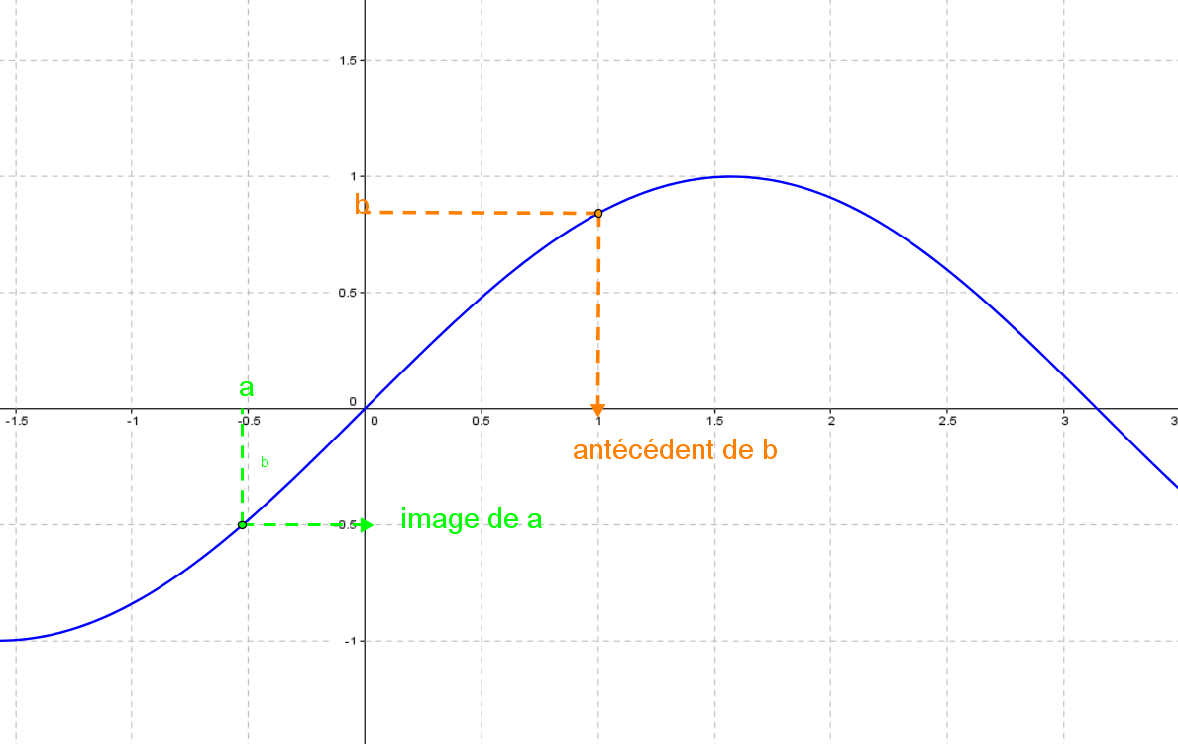
\includegraphics[scale=0.5]{./img/voc}
	\end{center}
	
	
	\subsection{Variations d'une fonction}
	
	\begin{mydefs}
		
		\begin{itemize}
			\item Si une fonction $f$ est \kw{croissante} sur un intervalle $I$ alors les images sont rangées dans le même ordre que leur antécédent ; c'est à dire que \kw{$f(x)$ augmente quand $x$ augmente}.
			\item Si une fonction $f$ est \kw{décroissante} sur un intervalle $I$ alors les images sont rangées dans l'ordre inverse de leur antécédent ; c'est à dire que \kw{$f(x)$ diminue quand $x$ augmente}.
		\end{itemize}
		
		
		%Si $f(x)$ augmente quand $x$ augmente, alors $f$ est \kw{croissante}.
		%Si $f(x)$ diminue quand $x$ augmente, alors $f$ est \kw{décroissante}.
	\end{mydefs}
	
	\newpage 
	
	\section{Fonctions linéaires, fonctions affines}
	
	\subsection{Définition}
	
	\begin{mydef}
		
		$a$ et $b$ sont des nombres quelconques ; la fonction qui à tout nombre $x$, associe le nombre \kw{$ax+b$}, est une \kw{fonction affine}.\\
		
		
		Cas particuliers :
		\begin{itemize}
			\item Si \kw{$b = 0$}, la fonction est \kw{linéaire}.
			\item Si \kw{$a=0$}, la fonction est \kw{constante}.
		\end{itemize}
	\end{mydef}
	
	\begin{myexs}
		On considère les fonctions $f,g,h$ et $i$ :
		\begin{multicols}{2}
			\begin{itemize}
				\item $f(x)=2x$
				\item $g(x)=-x+2$
				\item $h(x)=3x-4$
				\item $i(x)=5$
			\end{itemize}
		\end{multicols}
		
		\begin{itemize}
			\item $f$ est une fonction \kw{linéaire (On a $a=2$ et $b=0$)}.
			\item $g$ est une fonction \kw{affine (On a $a=-1$ et $b=2$)}.
			\item $h$ est une fonction \kw{affine (On a $a=3$ et $b=-4$)}.
			\item $i$ est une fonction \kw{constante (On a $a=0$ et $b=5$)}.
		\end{itemize}
	\end{myexs}
	
	\subsection{Représentation graphique}

	\begin{myprops}
		\begin{itemize}
			\item La \kw{représentation graphique} d'une fonction affine $f(x)=ax+b$ et \kw{une droite}. On dit que $y=ax+b$ est l'équation de la droite.
			\kw{a} est le \kw{coefficient directeur} (ou la pente) de la droite.
			\kw{b} est l'\kw{ordonnée à l'origine}.
			\item La droite passe par le point de coordonnées $(0;b)$, si la fonction est linéaire elle passe par l'origine du repère.
		\end{itemize}
		
	\end{myprops}
	
	\begin{myex}
		\begin{multicols}{2}
			\vspace*{1.5cm}
			On considère la fonction affine $f(x)=2x+4$. Elle ne passe pas par l'origine du repère, elle n'est pas linéaire. Elle passe par le point de coordonnées $(0;4)$.
			
			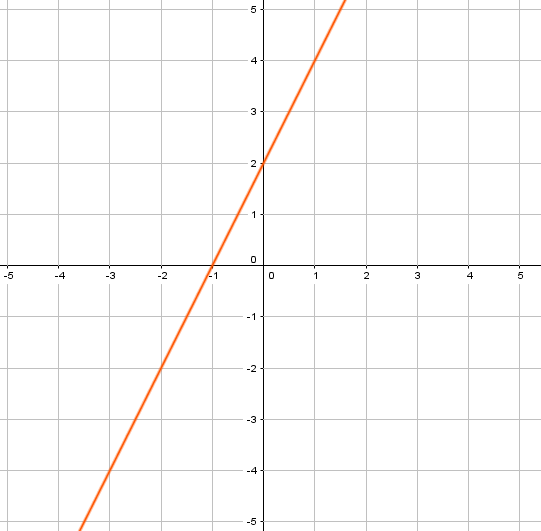
\includegraphics[scale=0.5]{img/ex1}
		\end{multicols}
	\end{myex}

	\subsection{Signe et variations}
	
	\begin{myprops}
		\begin{itemize}
			\item Si \kw{$x > \frac{- b}{a}$ } $f(x)$ est du \kw{signe de $a$}, si \kw{$  x < \frac{- b}{a} $}  elle est du \kw{signe contraire}.
			\item Si \kw{$a > 0$}, alors la fonction $f$ est \kw{strictement croissante}.
			\item Si \kw{$a < 0$}, alors la fonction $f$ est \kw{strictement décroissante}.
		\end{itemize}
	\end{myprops}

	\begin{multicols}{2}
		\begin{center}
			$a>0$
			
			\vspace*{0.5cm}
			
			\begin{variations}
				x & \mI & & \dfrac{-b}{a} & & \pI \\
				\filet
				f(x) & \ga - & \z & \dr+ \\				
			\end{variations}
			
			\vspace*{1cm}
			
			
			\begin{variations}
				x & \mI & &  & & \pI \\
				\filet
				\m{f(x)} & \h\ &  \c & \h\ \\				
			\end{variations}
		\end{center}
	
		\begin{center}
			$a<0$
			
			\vspace*{0.5cm}
			
			\begin{variations}
				x & \mI & & \dfrac{-b}{a} & & \pI \\
				\filet
				f(x) & \ga + & \z & \dr- \\				
			\end{variations}
			
			\vspace*{1cm}
			
			
			\begin{variations}
				x & \mI & &  & & \pI \\
				\filet
				\m{f(x)} & \h\ &  \d & \h\ \\				
			\end{variations}
		\end{center}
	\end{multicols}


%	\subsection{Détermination d'une équation de droite}
%	
%	\begin{mybilan}
%		
%		On détermine l'équation ($y=ax+b$) d'une droite à partir de deux points de cette droite $A(x_A; y_A)$ et $B(x_B; y_B)$.
%		
%		Le coefficient directeur $a$, est obtenu par le calcul suivant :
%		
%		\begin{align*}
%			a = \dfrac{y_B - x_A}{x_B - x_A}
%		\end{align*}
%		
%		
%		L'ordonnée à l'origine $b$ est obtenue en remplaçant $x$ et $y$ dans l'équation par les coordonnées d'un des points.
%		
%	\end{mybilan}
%
%	\begin{myex}
%		La droite $\Delta$ passe par les points de coordonnées $(2;5)$ et $(4;9)$, on a :
%		
%		\begin{align*}
%		a &= \frac{9-5}{4-2} \\
%		a &= \frac{4}{2} \\
%		a &= 2
%		\end{align*}
%		
%		Donc l'équation de la droite $\Delta$ est de la forme $y=2x+b$. Pour trouver $b$ on remplace $x$ et $y$ par les coordonnées de $A$, on a :
%		
%		\begin{align*}
%		y &= 2x+b \\
%		5 &= 2 \times 2 + b  \\
%		5 &= 4 + b\\
%		1 &= b
%		\end{align*}
%		
%		Donc $\Delta$ est la droite d'équation $y=2x+1$.
%	\end{myex}
\section{Fonction carré}
	
	\begin{mybilan}
		La \kw{fonction carré} est définie par \kw{$x \mapsto x^2$}.
		
		Elle est :
		\begin{itemize}
			\item définie sur $\intervOO{- \infty }{+ \infty}$.
			\item décroissante sur $\intervOF{- \infty}{0}$ et croissante sur $\intervFO{0}{+ \infty}$.
			%			\item Sa représentation graphique est une \kw{parabole}.
		\end{itemize}
	\end{mybilan}
	
	
	\section{Bonus : Figure incomplète (3 points) }

$ABCD$ est un carré qui a été en partie effacé. On veut tracer son symétrique par rapport au point $O$.

\begin{questions}
	\question[1] Sans compléter le carré $ABCD$, construire $A'B'C'D'$, son symétrique par raport à $O$.
	
	\question[2] \'Ecrire un programme de construction pour $A'B'C'D'$.
\end{questions}

\begin{center}
	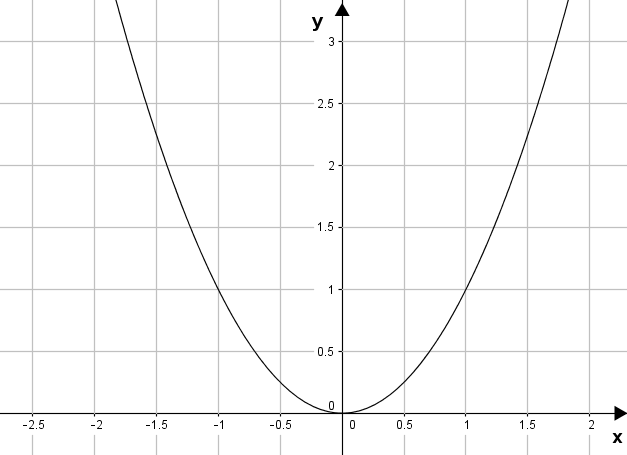
\includegraphics[scale=0.3]{img/carre}
\end{center}
	
	
	
	\section{Fonction inverse}
	
	\begin{mybilan}
		La \kw{fonction inverse} est définie par \kw{$x \mapsto \dfrac{1}{x}$}.			
		
		Elle est :
		\begin{itemize}
			\item définie sur $\intervOO{-\infty}{0} \cup \intervOO{0}{+\infty}$.
			\item décroissante sur $\intervOO{- \infty}{0}$ et sur $\intervOO{0}{+ \infty}$. 
			%			\item Sa représentation graphique est une \kw{hyperbole}.
		\end{itemize}
	\end{mybilan}
	
	
	\newpage
	
	\begin{myillus}

		Courbe représentative de la fonction $f(x) = \dfrac{1}{x}$ et tableau de variations associé:
	\begin{multicols}{2}

	


	\begin{center}
		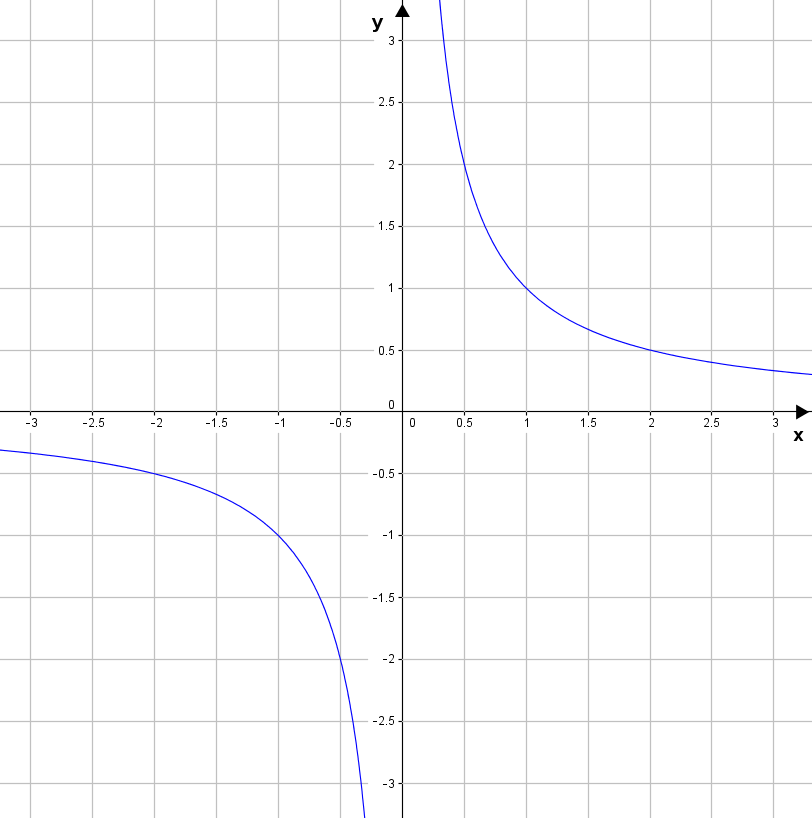
\includegraphics[scale=0.45]{./img/inverse}
	\end{center}
	
	

	\vspace*{1cm}
	\begin{center}
%		\begin{tikzpicture}
%		\tkzTabInit{$x$/1,$f(x)$/2}{$- \infty$,$0$,$+ \infty$}
%		%\tkzTabLine{,-,z,+}
%		\tkzTabVar{+/$+ \infty$,-/$0$,+/$+ \infty$}
%		\end{tikzpicture}	

		\begin{variations}
			x & \mI & & & 0 & & & \pI \\
		\filet
			\m{\dfrac{1}{x}} & \h\ & \d & \ & \bb & \h\ & \d & \ \\				
		\end{variations}
	\end{center}
	\end{multicols}
\end{myillus}
	
	\section{Fonction cube}
	
	
	\begin{mybilan}
		La \kw{fonction cube} est définie par \kw{$x \mapsto x^3$}.		
		
		Elle est définie et croissante sur l'intervalle $\intervOO{- \infty }{+ \infty}$.	
	\end{mybilan}
	
	
	\begin{myillus}

		Courbe représentative de la fonction $f(x) = x^3$ et tableau de variations associé:
	\begin{multicols}{2}

	


	\begin{center}
		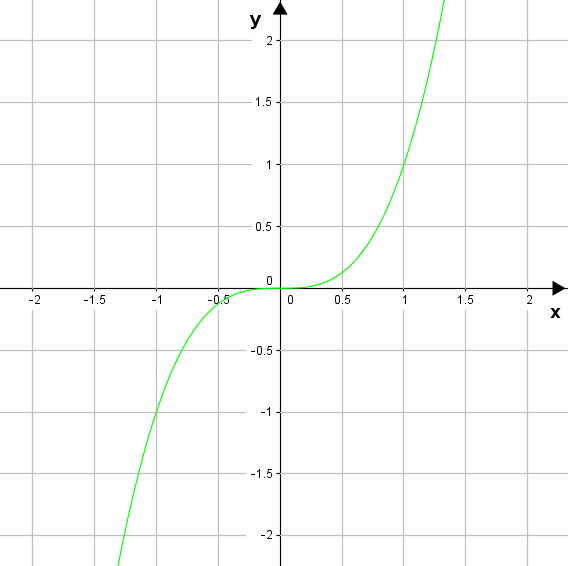
\includegraphics[scale=0.6]{./img/cube}
	\end{center}
	
	

	\vspace*{1cm}
	\begin{center}
%		\begin{tikzpicture}
%		\tkzTabInit{$x$/1,$f(x)$/2}{$- \infty$,$0$,$+ \infty$}
%		%\tkzTabLine{,-,z,+}
%		\tkzTabVar{+/$+ \infty$,-/$0$,+/$+ \infty$}
%		\end{tikzpicture}	

		\begin{variations}
			x & & \mI & & \pI \\
		\filet
			\m{x^3} & & \mI & \c & \h\pI \\				
		\end{variations}
	\end{center}
	\end{multicols}
\end{myillus}
	
	
	\section{Fonction racine}
	
	\begin{mybilan}
		La \kw{fonction racine carrée} est définie par \kw{$x \mapsto \sqrt{x}$}.			
		
		Elle est définie et croissante sur $\intervFO{0}{+\infty}$.
	\end{mybilan}
	
	
	%\begin{myillus}

		Courbe représentative de la fonction $f(x) = \sqrt{x}$ et tableau de variations associé:
	\begin{multicols}{2}

	


	\begin{center}
		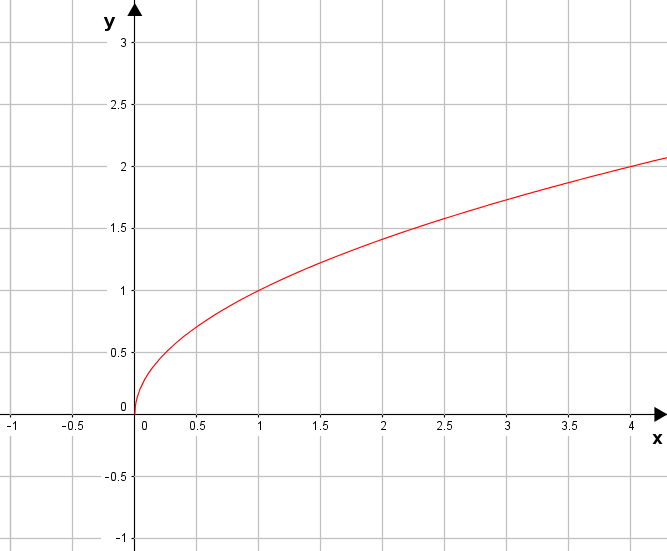
\includegraphics[scale=0.6]{./img/racine}
	\end{center}
	
	

	\vspace*{1cm}
	\begin{center}
%		\begin{tikzpicture}
%		\tkzTabInit{$x$/1,$f(x)$/2}{$- \infty$,$0$,$+ \infty$}
%		%\tkzTabLine{,-,z,+}
%		\tkzTabVar{+/$+ \infty$,-/$0$,+/$+ \infty$}
%		\end{tikzpicture}	

	\begin{variations}
		x & 0 & &  & & \pI \\
		\filet
		\sqrt{x} & & + &  \\				
	\end{variations}

	\vspace*{0.5cm}

		\begin{variations}
			x & & 0 & & \pI \\
		\filet
			\m{\sqrt{x}} & & \ & \c & \h\ \\				
		\end{variations}
	\end{center}
	\end{multicols}
%\end{myillus}
	
	
	
	
\end{document}